\documentclass[11pt]{article}
\usepackage[margin=1.1in]{geometry}
\usepackage{amsmath,amssymb}
\usepackage{enumitem}
\usepackage[hidelinks]{hyperref}
\usepackage{parskip}
\usepackage{graphicx}
\usepackage{booktabs}
\title{\vspace{-2em}\large\textbf{Feature-Funding Collapse on Scripted Data,\\ and Why the Same Mechanism Explains Multi-Modal Policy Consensus}}
\date{\normalsize July 17, 2026}
\author{}
\begin{document}
\maketitle
\vspace{-3em}

\section*{The scripted-data failure: a precise causal chain}

On the scripted data, the failure has a precise causal chain.

\begin{enumerate}[leftmargin=1.6em,itemsep=0.35em]
\item During the settle phase the actions are near-zero with essentially no local
variation, and they are fully predictable from the end-effector height alone ---
so the loss demands no other feature there, and training prunes the local
representation accordingly: the encoder's local Jacobian participation ratio --- the effective number of
input directions the encoder still responds to --- drops to ${\sim}1.5$--$4$ at settle versus $5$--$7$ in the moving phases
(from ${\sim}37$ at initialization).

\item The labels \emph{do} separate settle from the lift/transit stroke
on-support (97--99\% neighborhood purity, residuals at the noise floor), but
this separation is only as wide as fitting requires: the standard MSE loss's ($L_2$'s) separating
gradient is residual-proportional, so it decays to zero once the training
points are fit (measured: $+0.066$ early $\rightarrow$ $0.000$ at
convergence), and it is built asymmetrically, since settle's side pushes with
near-zero residuals.

\item The stroke passes through the same height band, so for any state
slightly off the demonstration support --- beyond the thin separator --- the
height coordinate, the only direction with retained gain, assigns it to
stroke content, and the policy reads out a full-magnitude translation during
the zero-tolerance grasp window. This is confirmed at the behavioral level:
the failure action matches the embedding-neighbor stroke labels
($\cos \approx +0.97$), and the quiet region's basin boundary sits at only
${\sim}40\%$ of the settle-to-stroke distance under $L_2$.

\item Hetero-Gaussian (HG; heteroscedastic Gaussian NLL with a learned per-sample scale $\sigma$) fixes this at the formation stage: its $1/\sigma^2$
weighting gives the near-zero-residual distinctions ${\sim}14\times$ the
relative gradient share (versus $0.19\times$ under $L_2$), keeping the
separating force alive after residuals shrink --- the settle region retains
${\sim}1.5\times$ more local feature directions, the basin boundary moves out
to ${\sim}60$--$70\%$, and the wrong-stroke readout stops being reachable in
closed loop.
\end{enumerate}

\section*{Relation to Multi-Modal Policy Consensus (arXiv:2509.23468)}

The multi-modality paper plausibly faces the same issue, transposed from the
phase axis to the modality axis. In contact-rich data, the tactile signal has
exactly the properties our settle phase has: it is informative only during
sparse contact windows (most of the time the touch channel is near-constant
--- the zero-local-variation condition), and on the clean training support it
is almost entirely redundant given vision --- the demonstrations can be fit
to the noise floor from visual features alone, just as our settle actions can
be regressed from the height axis alone. So nothing in a monolithic training
loss ever demands deep tactile features: gradient is allocated by explanatory
share on the training distribution, vision explains nearly all of it, and the
tactile directions of the fused representation are pruned the way our settle
chart is pruned. The separation this leaves behind is again only as wide as
fitting required --- and deployment queries the unpaid-for region: under
occlusion or perturbation, vision becomes ambiguous or misleading, and the
policy must answer from a state where only the pruned tactile features could
distinguish the right action. That is structurally identical to our drifted
settle states being assigned by the height coordinate: a representation
committed to the dominant channel, an off-support query, and a readout taken
from whatever content the retained coordinate matches --- which is why
``vision overwhelms sparse but critical touch'' is, in our terms, the
funding-starvation collapse occurring along the modality axis.


\section*{Supporting experiments and ablations (scripted data)}

\subsection*{Link 1 --- pruning of the settle chart (Fig.~\ref{fig:pr})}
The encoder's local feature richness is measured as the participation ratio
(PR) of the local Jacobian's squared singular values --- effectively, how many
input directions the encoder still responds to at a given state. We compare
\emph{quiet} training states (small position-action magnitude, e.g.\ settle)
against \emph{loud} ones (large motions), for four losses: $L_2$ (plain MSE),
HG and HT (heteroscedastic Gaussian and Student-$t$: a network head predicts a
per-sample scale $\sigma(x)$, so the loss weights each sample by
$1/\sigma^2$), and MIP (the two-view denoising flow-map objective our project
studies). Training \emph{prunes} all charts from a rich initialization; the
losses differ in where the quiet window's pruning floor lands. Causal controls: removing the height coordinate
costs every model $0.36$--$0.72$ of its function (all other groups $\le
0.04$); curated observations give the \emph{same} collapse depth onto an
unambiguous coordinate and a success rate (SR) of $100/100$ ($\times 3$ seeds) --- the disease
requires the ambiguous survivor, not the collapse.

\begin{figure}[h]\centering
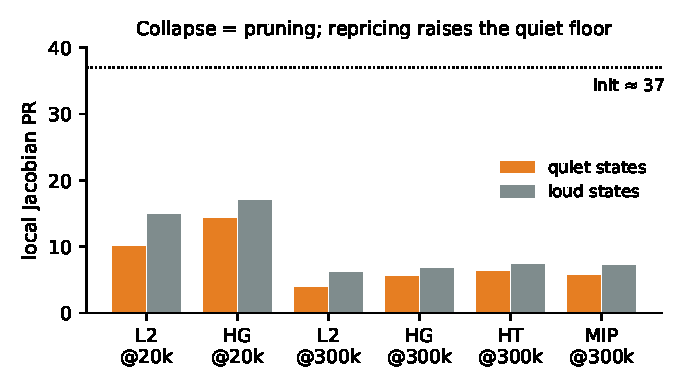
\includegraphics[width=0.62\linewidth]{figs/fig_pr.pdf}
\caption{Quiet-vs-loud local PR across losses and training stages.}
\label{fig:pr}
\end{figure}

\subsection*{Link 2 --- separation is only as wide as fitting requires (Table~\ref{tab:sep})}

\begin{table}[h]\centering\small
\begin{tabular}{lcc}
\toprule
 & $L_2$ & repriced / anchored \\
\midrule
on-support neighborhood purity & 97--99\% & 97--99\% \\
teacher-forced residual (floor) & $0.0016$ & $0.0008$ \\
separating force, 39k $\to$ 300k & $+0.066 \to 0.000$ & MIP retains $+0.15$ \\
merge cost, label-similar pairs & $\approx$ free ($0.95$) & $13\times$ \\
off-tube settle purity ($d\ge2$) & 3\% & 0--7\% (universal) \\
\bottomrule
\end{tabular}
\caption{Supervision separates the training points for every loss; only the
repriced losses (HG/HT) and the anchored one (MIP) keep paying for the margin
after residuals reach the floor. ``Off-tube'' means normalized distance
$d\ge 2$ from the nearest demonstration state, i.e.\ off the data support.
The off-tube fold is universal --- the failure site, not the cause.}
\label{tab:sep}
\end{table}

\noindent\emph{Intervention control:} shortening the training chunk horizon to $H{=}2$ changes which states share targets; there, where the target geometry
changes, the fold moves to the newly colliding pairs
(settle$\to$approach $79\%$, shoulder$\to$post $89\%$; healthy $H{=}10$
control) --- the learned metric follows the labels by construction.

\subsection*{Link 3 --- off-support readout and its execution dependence (Fig.~\ref{fig:basin})}
The failure action equals the embedding-neighbor label mean
($\cos \approx +0.97$; zero alignment to observation-space neighbors), and
canonicalizing the gripper coordinate collapses the cross-phase assignment
($62\% \to 1\%$). Fig.~\ref{fig:basin} (left) shows the basin geometry; the right panel shows that the wrong readout costs success only when
executed open-loop (per-cycle windows: $L_2$ corrective-head/expansive-tail
$-0.17/-0.17/{+0.08}$ vs.\ HG monotone contraction $-0.28/-0.35/-0.42$).

\begin{figure}[h]\centering
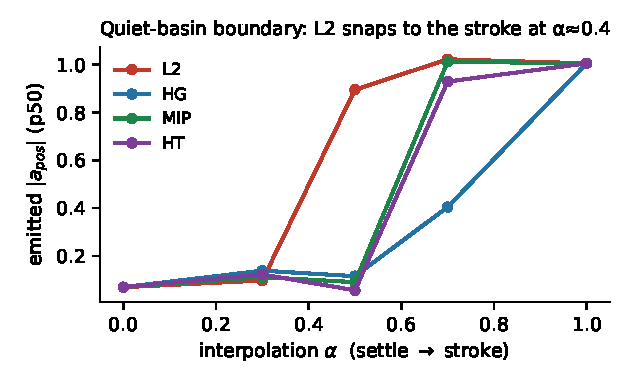
\includegraphics[width=0.48\linewidth]{figs/fig_basin.pdf}\hfill
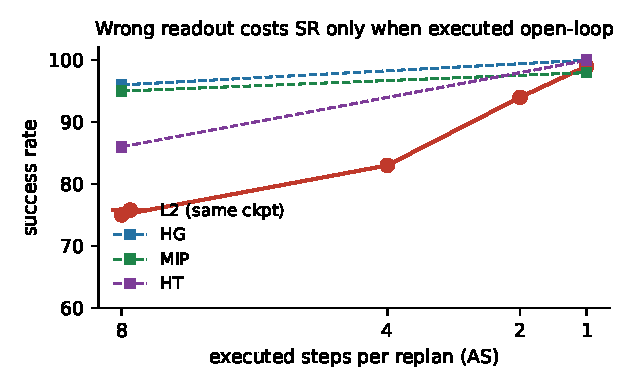
\includegraphics[width=0.48\linewidth]{figs/fig_as.pdf}
\caption{Left: emitted action magnitude along the settle$\to$stroke
interpolation. Right: success vs.\ executed steps per replan (same
checkpoints).}
\label{fig:basin}
\end{figure}

\subsection*{Link 4 --- the hetero-Gaussian mechanism and outcomes (Fig.~\ref{fig:sigma}, Tables~\ref{tab:seeds},~\ref{tab:controls})}

\begin{figure}[h]\centering
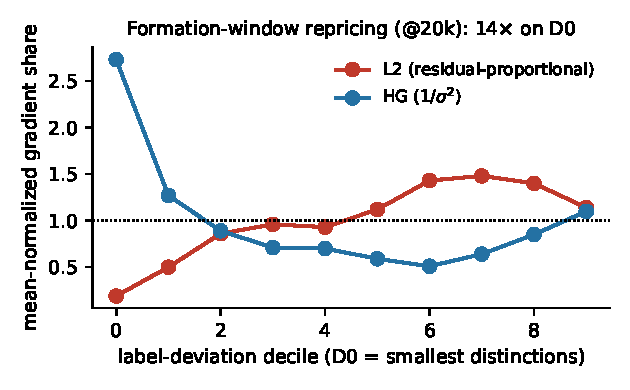
\includegraphics[width=0.6\linewidth]{figs/fig_sigma.pdf}
\caption{Gradient share by label-deviation decile at the 20k snapshot:
$1/\sigma^2$ re-prices the smallest distinctions $14\times$ relative to
$L_2$ and suppresses the outlier pocket; $\sigma$ collapses to its floor by
300k (a formation-window channel).}
\label{fig:sigma}
\end{figure}

\begin{table}[h]\centering\small
\begin{tabular}{lcc}
\toprule
3 training seeds & AS$=8$ (standard) & AS$=1$ \\
\midrule
$L_2$            & $\{75, 66, 70\}$ & $\{98, 75, 92\}$ \\
hetero-Gaussian  & $\{96, 97, 88\}$ & $\{100, 95, 95\}$ \\
$L_2$ 3-seed ensemble & $83$ & $96$ \\
\bottomrule
\end{tabular}
\caption{Seed families are disjoint at the standard protocol: repricing acts
as a \emph{selector} (variance collapse), not only a mean shift. The
checkpoint ensemble recovers about half the gap (posterior averaging).}
\label{tab:seeds}
\end{table}

\begin{table}[h]\centering\small
\begin{tabular}{llc}
\toprule
intervention family & example (SR) & verdict \\
\midrule
static reweighting & Cauchy 57; residual-w.\ 66; rel-err 72 & fails \\
representation regularizers & contrastive 8; isotropy 2--19; isometry 86$^{*}$ & fails \\
smoothing / Jacobian penalties & obs-noise 68; jacreg 1--24 & fails \\
adaptive repricing ($1/\sigma^2$) & hetero-Gaussian 96 & \textbf{works} \\
label-variation injection & progaux ($L_2$ + episode-progress output) 94 & works \\
observation curation & minimal (16-dim curated obs) 100 & works \\
short-horizon ladder ($H{=}2$) & $L_2$ 71 / MIP 81 / HG 91 & ordered by repricing strength \\
\bottomrule
\end{tabular}
\caption{Specificity controls. $^{*}$stressreg attains the flattest geometry
measured yet leaves the fold intact --- rank without content does not cure.}
\label{tab:controls}
\end{table}


\section*{How each step of the explanation is established}

\subsection*{Q2 first: does the representation actually collapse, and how is that measured?}
Collapse is measured on the trained encoder, per state, by three quantities:
the participation ratio (PR) of the local Jacobian's squared singular values
--- the effective number of input directions the encoder responds to; the
condition-number--style ratio $\kappa_{10} = s_1/s_{10}$ (how dominant the
top direction is over the tenth); and the largest input column's share of the
Jacobian's Frobenius mass. Table~\ref{tab:collapse} collects the
measurements. Reading it: the encoder starts isotropic (PR $\approx 37$);
$L_2$ training prunes the \emph{quiet} states' chart far harder than the loud
states' (PR $3.8$ vs.\ $6.1$; $\kappa_{10}$ $8.3$ vs.\ $4.8$ --- and at the
narrow settle band itself, PR $1.6$ with $\kappa_{10} \approx 12.6$); the
snapshots show this is monotone pruning of an initially rich chart, already
under way at 20k; and the repriced losses end with both a higher quiet floor
and a smaller quiet-vs-loud asymmetry. The surviving direction under $L_2$ is
a height composite spread over ${\sim}12$ redundant static-object columns
(pairwise $|\cos| = 0.89$), which is why the top-column share stays low even
as the chart collapses --- the committed feature hides across many correlated
columns rather than in one.

\begin{table}[h]\centering\small
\begin{tabular}{lcccccc}
\toprule
 & \multicolumn{2}{c}{PR} & \multicolumn{2}{c}{$\kappa_{10}$} & \multicolumn{2}{c}{top-column share} \\
checkpoint & quiet & loud & quiet & loud & quiet & loud \\
\midrule
initialization            & \multicolumn{2}{c}{$\approx 37$ (isotropic)} & --- & --- & --- & --- \\
$L_2$ @20k                & 10.1 & 14.9 & 3.6 & 2.8 & .05 & .04 \\
$L_2$ @300k               & \textbf{3.8} & 6.1 & \textbf{8.3} & 4.8 & .07 & .05 \\
\quad settle band only    & \textbf{1.6} & --- & $\approx$\textbf{12.6} & --- & --- & --- \\
HG @20k                   & 14.2 & 17.0 & 2.9 & 2.6 & .04 & .03 \\
HG @60k                   & 8.3 & 10.5 & 4.1 & 3.4 & .05 & .04 \\
HG @300k                  & 5.5 & 6.7 & 5.7 & 4.5 & .06 & .05 \\
HT @300k                  & 6.3 & 7.3 & 5.1 & 4.3 & .05 & .05 \\
MIP @300k                 & 5.7 & 7.2 & 5.3 & 4.3 & .07 & .05 \\
\midrule
tool-hang \emph{human}, $L_2$ & 16.4 & 18.1 & 2.5 & 2.3 & .03 & .03 \\
\bottomrule
\end{tabular}
\caption{Collapse measurements: local Jacobian PR, $\kappa_{10}$, and
top-column Frobenius share at quiet vs.\ loud training states. ``Quiet'' =
position-action magnitude below the 40th percentile; ``settle band'' = the
narrow grasp-alignment window only. The human-data row is the negative
control: where quiet windows carry label variation, no quiet-vs-loud
collapse gap forms.}
\label{tab:collapse}
\end{table}

\subsection*{Q1: how do we know the collapse is caused by the claimed cause?}
The claimed cause is the absence of local label variation (nothing demands
that the output change with the state there) combined with $L_2$'s
residual-proportional allocation. Three interventions isolate it:
\begin{itemize}[leftmargin=1.5em,itemsep=0.2em]
\item \textbf{Manipulate label variation, hold everything else fixed:}
injecting $5$\,mm of label noise raises settle richness $1.9 \to 4.1$; human
tremor (natural variation) gives $5.6$--$5.9$, and the trained human encoder
shows no quiet-vs-loud gap at all (last row of Table~\ref{tab:collapse});
the collapse tracks the variation dose and appears \emph{only} where labels are locally constant
(per-phase map matches the label-variation map; human datasets show no
quiet-vs-loud gap).
\item \textbf{Manipulate the allocation, hold the data fixed:} replacing
$L_2$ by the $1/\sigma^2$-weighted loss --- whose funding shift we verify
directly in the gradient tables ($14\times$ relative share on the smallest
distinctions at 20k) --- raises the quiet pruning floor $3.8 \to 5.5$ on
identical data. Same data, different funding, different collapse depth.
\item \textbf{Localization control:} the collapse sits exactly at the states
whose labels are quiet, at every loss, in proportion to that loss's residual
funding (quiet/loud PR ratio $0.62$ for $L_2$ vs.\ $0.79$--$0.86$ repriced; Table~\ref{tab:collapse}).
\end{itemize}

\subsection*{Q3: how does the collapse influence success rate?}
Not directly --- and the factor-isolation experiments are the point. Collapse
harms SR only in conjunction with two other factors: an \emph{ambiguous}
surviving coordinate, and \emph{open-loop exposure} of the off-support
region. Each factor is switched off separately while the others are held:

\begin{table}[h]\centering\small
\begin{tabular}{cccc}
\toprule
collapse & ambiguous survivor & executed open-loop & SR \\
\midrule
yes & yes & yes & $71$--$75$ \quad (full-obs $L_2$, AS$=8$) \\
yes & \textbf{no} & yes & $100$ \quad (curated obs; same collapse depth) \\
yes & yes & \textbf{no} & $99$ \quad (same checkpoint, AS$=1$) \\
\textbf{reduced} & yes & yes & $94$--$96$ \quad (repriced loss) \\
\bottomrule
\end{tabular}
\caption{Factor isolation: switching off any single factor removes the SR
damage. The collapse influences SR only through the chain collapse $\times$
ambiguity $\rightarrow$ off-support misassignment $\rightarrow$ wrong
full-magnitude readout $\rightarrow$ executed open-loop.}
\label{tab:factors}
\end{table}

The mediation is quantified: at the policy's own off-support states the
neighborhood purity drops to $3\%$ and the emitted action equals the
neighbor-label mean ($\cos +0.97$); success is then monotone in the escape
rate across all five losses (escape fraction
$0.29/0.19/0.11/0.07/0.06 \rightarrow$ SR $75/86/94/95/96$). Two cautions
keep the claim honest: richness is a \emph{footprint} of funding, not itself
sufficient (the flattest-geometry regularizer scores only $86$ with the
misassignment intact, and the richest-chart repriced loss is the weakest of
the three winners), and the same conjunction predicts \emph{absence} of harm
correctly --- on human data, where quiet windows carry label variation, no
collapse forms and the failure modes are entirely different.

\paragraph{Known limitations.} The $H{=}2$ ladder and some matrix cells are
single training seed (evaluation-seed replicated only); baseline horizons are
$H{=}10$; whether the hetero-Gaussian effect flows through the transient
weighting path or the $\sigma$-head's feature shaping is under test (a
decoupled control is being evaluated).

\end{document}
